%!TEX root = ../template.tex
%%%%%%%%%%%%%%%%%%%%%%%%%%%%%%%%%%%%%%%%%%%%%%%%%%%%%%%%%%%%%%%%%%%%
%% chapter5.tex
%% NOVA thesis document file
%%
%% Chapter with lots of dummy text
%%%%%%%%%%%%%%%%%%%%%%%%%%%%%%%%%%%%%%%%%%%%%%%%%%%%%%%%%%%%%%%%%%%%
\chapter{Desenvolvimento}
O desenvolvimento do projeto pode ser dividido de grosso modo em três camadas. Nelas são cobertos um grupo abrangente de aspetos tanto da área do processamento de linguagens e do desenvolvimento de \acrshort{dsl}'s, da teoria músical, e do processamento digital de audio. 

Na camada da linguagem esteve mais proeminente a área de processamento de linguagens, por motivos óbvios. Mas nas decisões tomadas durante o desenvolvimento desta camada, estiveram sempre presentes também as necessidades específicas que a teoria músical (e a sua notação) impõeem numa linguagem de programação.

Do mesmo modo, o interpretador faz claramente uso de tópicos do domínio do processamento de linguagens, mas é ainda mais fortemente influencidado pelas restrições  e requisitos impostos pela componente músical da linguagem. Esta influencia a forma e a semântica da execução dos vários operadores disponibilizados.

A última camada, de desenvolvimento de uma biblioteca, composta pelos objetos e procedimentos que têm como objetivo facilitar a utilização da linguagem. Para isso foi necessário identificar os casos de utilização mais comuns e prioritários, de modo a guiar a construção destas interfaces para refletirem uma utilização real da aplicação.

\section{Linguagem}
A camada sintática da aplicação pode ser conceptualmente dividida em duas fases:
\begin{description}
    \item[Sintaxe] Esta fase caracteriza-se por delinear qual a sintaxe usada pela linguagem, bem como os construtores e operadores suportados;
    \item[Parser] Nesta fase foi desenvolvido um \textit{parser} em \textit{Python}, responsável por converter o código fonte da linguagem numa \acrfull{ast};
\end{description}

No entanto, a realidade é que a abordagem seguida (não só nesta camada mas como em todo o projeto) foi mais iterativa, dividindo cada faze em porções semi-independentes e intercalando as várias porções das diversas fases. Esta abordagem tem a vantagem de permitir ir testando e experimentando com o projeto mais cedo do que seria possível com um modelo de desenvolvimento em cascata.
\subsection{Sintaxe}
A sintaxe da linguagem é bastante inspirada nas usualmente chamadas linguagens da família C, com recurso a parênteses curvos e chavetas para delínear os vários blocos da linguagem. No entanto, as expressões são complementadas com um novo conjunto de literais e operadores dedicados a componente músical da linguagem. Conseguir juntar estes dois mundos trás consigo alguns desafios que serão discutidos mais em detalhe em cada umas das secções seguintes.

\subsubsection{\textbf{Literais}}
Literais referem-se ao conceito de sintaxe desenhada com o propósito de descrever data (literal) no código. São usados em quase todas as linguagens de programação (e na nossa também) para descrever números, \textit{strings} e booleanos.

A maior diferença nesta área entre a nossa linguagem foi a adição de literais responsáveis por modelar conceitos músicais, como notas, pausas e acordes. Esta sintaxe, tal como já foi mencionado anteriormente, foi inspirada pelo projecto \textit{abc notation}, com algumas modificações.

\subsubsection{\textbf{Notas e Pausas}}
A sintaxe de notas descrição de notas é composta por quatro componentes: \textbf{acidentais}, \textbf{\textit{pitch}} (obrigatório), \textbf{oitava} e \textbf{duração}.

\begin{lstlisting}[caption=Expressão regular que identifica uma nota (quebras de linha apenas para claridade de leitura)]
[_^]*
[a-gA-G]
[',]*
([0-9]*\/)?[0-9]*
\end{lstlisting}

O \textit{pitch} refere-se à nota (ou frequência) que deve ser tocada. O \textbf{C médio} (também conhecido como C4) é descrito simplesmente como \texttt{C}. É possível descer uma ou mais oitavas acrescentando uma ou mais vírgulas \texttt{,}. Para subir uma oitava, podemos primeiro substituir as letras maíusculas por minúsculas. Para subir mais oitavas, podemos acrescentar uma ou mais pelicas \texttt{'}. Para subir ou descer semitons, podemos preceder a notas com os acidentais \texttt{\_} e \texttt{\^}.

As pausas são mais simples, sendo compostas simplesmente pela letra \texttt{r} seguida da sua \textbf{duração} (usando as mesma sintaxe das notas).

\subsubsection{\textbf{Acordes}}
Para definir acordes na linguagem, colocam-se várias notas dentro de parenteses retos. A notação usada para cada nota inclui os seus três primeiros componentes (acidentais, \textit{pitch} e oitava), mas exclui a duração. Em vez de definir a duração em cada nota, esta é definida globalmente no acorde após fechar os parenteses retos.

Por conveniência, para evitar ao utilizador ter de introduzir todas as notas de um acorde manualmente, temos uma sintaxe abreviada para os tipos de acordes mais comuns, onde é apenas necessário introduzir a nota base seguido do tipo de acorde.

\begin{table}[h]
\centering
\def\arraystretch{1.3}
\begin{tabular}{|l|c|}
\hline
\textbf{}        & \textbf{Abreviações}           \\ \hline
\textbf{Tríades} & M, m, aug, dim, +                \\ \hline
\textbf{Quinta}  & 5                                \\ \hline
\textbf{Sétimas} & m7, M7, dom7, 7, m7b5, dim7, mM7 \\ \hline
\end{tabular}
\caption{Lista de abreviaturas possíveis de serem acrescentadas a seguir a uma nota para especificar um acorde.}
\label{tab:modifiers-list}
\end{table}

A decisão de envolver cada acorde com parênteses retos deveu-se ao facto de muitas abreviaturas serem já populares no domínio da notação músical, e como tal o ideal era não as mudar. No entanto, algumas dessas abreviaturas poderiam entrar em conflito com outros componentes da declaração da nota. Por exemplo, \texttt{C7} poderia ser tanto um acorde de sétima como uma nota com duração de 7. Com a separação por parenteses retos, a ambiguidade deixa de existir, sendo obvio que \texttt{[C7]} é um acorde de sétima, e \texttt{C7} é uma nota com duração 7.

\begin{lstlisting}[caption={Exemplos de três definições de acordes possíveis}] 
[CFG]/4 [^Fm] [C5]2
\end{lstlisting}

\subsubsection{\textbf{Modificadores}}

Para além de permitir descrever notas, também é possível ter modificadores de contexto que permitem alterar certas propriedades das notas e acordes. Duas destas propriedades (duração e oitava) podem ser depois customizadas em cada nota ou acorde, como já vimos. No entanto, em vez de estes valores substituirem simplesmente os valores predefinidos, eles ``complementam-se''.

Ou seja, se declarar-mos por exemplo que a duração base das notas é $\frac{1}{4}$. Quando definirmos alguma nota a seguir com a duração de $\frac{1}{2}$, a sua duração real irá ser calculada da seguinte forma $\frac{1}{4} \times \frac{1}{2} = \frac{1}{8}$.

Do mesmo modo, quando definimos por exemplo a oitava base como $5$ (o valor predefinido é $4$), a nota \texttt{C,} passa a representar a oitava $5 - 1 = 4$ (por predefinição seria $4 - 1 = 3$).

Podemos então ver a lista dos modificadores aceites pela linguagem, bem como exemplos de utilização e os seus respetivos valores predefinidos (usados quando nenhum modificador é aplicado).

\begin{table}[h]
\centering
\def\arraystretch{1.3}
\begin{tabular}{|l|c|c|c|}
\hline
\textbf{Nome} & \textbf{Modificador}                                            & \textbf{Exemplo}                                        & \textbf{Predefinição} \\ \hline
Instrumento   & I$N$                                                            & I46                                                     & I0           \\ \hline
Velocidade    & V$N$                                                            & V100                                                    & V127         \\ \hline
Tempo         & T$N$                                                            & T120                                                    & T60          \\ \hline
Duração       & \begin{tabular}[c]{@{}c@{}}L$N$\\ L/$N$\\ L$D$/$N$\end{tabular} & \begin{tabular}[c]{@{}c@{}}L2\\ L/4\\ L3/8\end{tabular} & L1           \\ \hline
Oitava        & O$N$                                                            & O2                                                      & O4           \\ \hline
Compasso      & S$D$/$N$                                                        & S3/4                                                    & S4/4         \\ \hline
\end{tabular}
\caption{Lista de modificadores e exemplos da sua utilização}
\label{tab:modifiers-list}
\end{table}

\subsubsection{\textbf{Variáveis e Funções}}
Uma das consequências da introdução da sintaxe de notas literais foi a impossibilidade de ter variáveis com certos nomes. Uma variável chamada \texttt{a}, por exemplo, iria entrar em conflito com a nota do mesmo nome. Do mesmo modo, uma variável chamada \texttt{i1} iria entrar em conflito com o modificador de instrumento. 

Em vez de criar casos de excepção para as variáveis que possam ter nomes que conflitam com outros construtores sintáticos, seguimos o exemplo de outras linguagems como \textit{PHP}, \textit{Perl} ou \textit{Powershell}, e decidimos prefixar as nossas variáveis com o caracter \texttt{\$}.

No caso das funções foi possível evitar a ambiguidade (e do mesmo modo a obrigatoriedade de as prefixar com um caracter) devido ao facto de as funções terem obriugatoriamente um par de parênteses (sem espaço entre o nome da função) quando são chamadas.

No entanto não quer dizer que as funções passaram imunes à introdução das literais de música. Uma vez que a vírgula é usada para mudar a oitava de uma nota (e foi escolhida de forma a manter compatibilidade com a sintaxe do projeto \textit{abc notation}, existem casos em que esta não pode ser utilizada para separar os argumentos passados a uma função.

Por exemplo, dada a expressão \texttt{function\_name(C, A, \$a, 2)}, podemos concluir que a mesma tem quantos argumentos? A resposta correta seria dois, pois as duas primeiras vírgulas poderiam pertencer à nota ou ao separador da função. Mas neste caso a nota teria prioridade, pelo que \texttt{C, A, \$a} seria o primeiro argumento, e \texttt{2} seria o segundo.

A solução tomada inicialmente foi utilizar ponto-e-vírgula para substituir a vírgula como separador de argumentos  nas funções. E enquanto iso resolveu os problemas de ambiguidade, tornou-se óbvio à medida que que a linguagem foi avançando, que a prevalência da vírgula como separador em quase todas as linguagens de programação mais populares fazia com que houvesse um custo mental de mudança de contexto sempre que alguém mudava de alguma linguagem para a nossa, e vice-versa.

A solução escolhida no final foi um compromisso entre as duas opções: tanto a vírgula como o ponto-e-vírgula podem ser usados como separadores de argumentos, com a exceção de quando o argumento é uma nota músical, onde o ponto-e-vírgula tem de ser obrigatoriamente usado. Assim sendo, poderiamos rescrever o exemplo anterior da seguinte forma \texttt{function\_name(C; A; \$a, 2)}, passando a função a receber agora os quatro argumentos como seria inicialmente esperado.

\subsection{Parser}
Para implementar o parser da linguagem, foi utilizado o módulo \textit{Python} \textbf{Arpeggio}, um módulo que implementa um algoritmo de \textit{parsing} descendente recursivo como recurso a \textit{memoization} para melhora da performance. A gramática utilizada pode ser vista em maior detalhe no apêndice \ref{grammar}.

\begin{lstlisting}[caption={Excerto da gramática desenvolvida}]
main <- body EOF;

body <- statement ( ";" statement )* _ ";"? _
    / ""
    ;

// Statements
statement <- _ ( var_declaration / voice_declaration / function_declaration / for_loop_statement / while_loop_statement / if_statement / expression ) _;

var_declaration <- "$" namespaced _ "=" _ expression;
// ...
\end{lstlisting}

A gramática PEG desenvolvida para o projeto foi depois complementada por uma classe \textbf{Parser}, responsável por gerar a \acrshort{ast} da linguagem. Para isso recorremos ao \textit{Visitor Pattern}, com um método para cada regra não-terminal da gramática (todos prefixados com \texttt{visit\_}).

\begin{lstlisting}[caption={Métodos responsáveis por criarem a AST}]
def visit_body ( self, node, children ): ...

def visit_comment ( self, node, children ): ...

def visit_statement ( self, node, children ): ...

def visit_var_declaration ( self, node, children ): ...
\end{lstlisting}

\section{Interpretador}
As linguagens compiladas usualmente recorrem à compilação \acrfull{aot}, em que o código é transformado em código máquina com antecedência (durante a fase de compilação). Esta é a solição que consegue geralmente oferecer melhor \textit{performance}, menor consumo de memória e tempos de \textit{startup} mais rápido. Por outro lado, obriga a um passo de compilação separado sempre que o código fonte é alterado, e regra geral necessita de tipos de dados estáticos.
No que toca a linguagens interpretadas temos mais opções. Podemos então dividir os seus modos de execução em três categorias distintas, cada uma com possíveis vantagens e desvantagens, bem como diferenças de dificuldade de implementação bastante salientes.
\begin{description}
 \item[Interpretadores] Também chamados por vezes como interpretadores \textit{tree walk}, são usualmente os mais simples de implementar (mas também os mais lentos a executar). O seu conceito baseia-se no \textit{design pattern} homónimo, em que as operações da linguagem são modeladas numa árvore, geralmente igual ou similar à estrutura da \acrshort{ast}. Para executar uma expressão é chamado um método na raiz da árvore, e esse método irá chamar recursivamente os métodos das suas sub-expressões, passando o estado como argumentos da função, e recebendo o resultado pelo valor retornado da função.
 \item[Bytecode VM] São chamadas máquinas virtuais (VM) porque o seu comportamento assemelha-se mais ao comportamento dos processadores reais dos computadores. As expressões da árvore de sintaxe abstrata são previamente convertidas numa sequência linear de instruções mais simples (geralmente compactadas em binário para melhor \textit{performance}, também referido como \textit{bytecode}. Cada instrução é depois executada dentro de um ciclo. Esta solução fornece um balanço entre facilidade de implementação e velocidade de execução (evitando a grande quantidade de chamadas recursivas de funções presentes nos interpretadores).
 \item[Just In Time] O método mais complexo (mas também o que oferece melhor \textit{performance} para tarefas pesadas). O código é executado inicialmente por um dos dois métodos anteriores, de modo a recolher estatísticas sobre qual o tipo de execução mais comum do código. Após esta recolha, é gerado código máquina optimizado para os tipos de dados mais comuns de uma variável, ou para os caminhos de execução mais prevalentes, para que seja possível da próxima vez que o mesmo pedaço de código seja executado, isso ocorra com recurso ao código máquina. Este processo é gerlamente repetido ao longo da execução do programa, sendo que caso a versão de código máquina gerada fique desatualizado (o tipo de dados usualmente passados a uma função mudem), essa porção de código seja invalidada e eventualmente substituida por uma nova versão mais adequada.
 \end{description}

 É possível ver que a solução ideal seria sempre a compilação \acrfull{jit}, que evita uma fase de compilação explícita e forçada ao utilizador, mas ao mesmo tempo consegue fornecer \textit{performance} competitiva para tarefas mais exigentes. No entanto é inevitável concluir que esta solução impõe custos de desenvolvimento astronómicos, e implica equipas de grande dimensão e tempos de desenvolvimento extremamente longos.
 
 Desta forma a nossa escolha reside logicamente entre a solução de \textbf{Interpretador} e um simples \textbf{Bytecode}. Acabamos por escolher a primeira opção pelas seguintes razões:
 \begin{itemize}
  \item A geração de eventos músicais é relativamente computacionalmente barata (mesmo admitindo algumas dezenas de eventos músicais por segundo).
  \item A componente mais pesada geralmente reside na sintetização dos eventos músicais (\textit{note on, note off}) em \textit{streams} de audio, mas esta tarefa é encaminhada para bibliotecas desenvolvidas em linguagens de baixo nível.
  \item A possibilidade de correr código \textit{Python} no meio de qualquer parte da nossa linguagem já fornece um bom meio termo para quando é necessária mais alguma \textit{performance} (sem sacrificar demasiado a simplicidade de uma linguagem destinada primariamente a músicos e não engenheiros informáticos).
  \item Também a facilidade de implementação de um interpretador significou uma velocidade de ordens de magnitude superior durante a implementação da linguagem e da prototipação de funcionalidades.
  \item Uma posterior modificação do interpretador para uma \textit{bytecode VM} mais eficiente seria possível estando a linguagem mais estabilizada, e seria simples manter uma \acrshort{api} virtualmente 100\% compatível.
 \end{itemize}

 Em conclusão, cada operação foi implementada através de um método \texttt{eval()} em cada classe da \acrshort{ast}, recebendo uma variável de contexto como \textit{input}, e usando depois o valor retornado pela função como resultado da avaliação da expressão.
 
\subsection{Contexto}
A variável de contexto guarda o estado da execução, e deve conter toda a informação necessária para cada instrução poder executar. Os seus conteúdos podem ser divididos em três componentes:
\begin{description}
 \item[Timestamp] Esta propriedade é um simples inteiro que permite às expressões de geração de eventos músicais saberem qual o tempo virtual atual. Este tempo virtual é manipulado pelos vários operadores. O operador sequencial por exemplo, que recebe uma lista de expressões e emite uma lista de eventos músicais uns a seguir aos outros, avança este cursor para o fim do último evento antes de passar o contexto para avaliar a expressão seguinte.
 \item[Voz] Objeto que contém as várias propriedades músicais que devem ser aplicadas durante a geração de eventos, tais como a duração base das notas, o compasso ou as batidas por minuto.
 \item[Símbolos] Um contentor que permite aceder e modificar os símbolos disponíveis na linguagem (tais como variáveis e funções).
 \end{description}
 
 Os contextos foram desenhados com o intuito de serem leves, daí apenas conterem  referências para três variáveis. Desta forma é possível criar cópias dos contextos e permitir que operações variadas estejam a executar ao mesmo tempo com diferentes contextos.
 
 Para percebermos a razão desta necessidade, basta pensarmos no operador paralelo. Se colocarmos duas expressões músicais que devem tocar ao mesmo tempo, a geração de uma (ou mais) notas na primeira expressão não deve afetar o \texttt{timestamp} da segunda. Para isto, cada uma das expressões deve receber uma cópia do contexto (com o \textit{timestamp} inicial igual). Quando as duas expressões terminarem, no entanto, é importante que o contexto original (que gerou as duas cópias) atualize os seu \textit{timestamp} para qual for a expressão mais longa.
 
 Se prestarmos atenção, podemos estar aqui a detetar um padrão bastante comum na área da programação: o modelo \textbf{fork-join}.
 
 E é fácil perceber que faz sentido. Apesar de estarmos a lidar com notas e eventos músicais, fundamentalmente estamos a criar ramos paralelos de execução, e queremos no final aguardar o seu resutado e uníficá-lo com o ramo original. Se substituirmos ramo por \textit{thread} para o caso da programação, ou \textit{contexto} para o nosso caso, vemos a equivalência de contextos.
 
 Como tal, para além do estado (as três variáveis) que o objeto de contexto engloba, este providencia também algumas operações bastante simples e úteis:
 
 \begin{description}
  \item[Fork] Cria uma cópia do contexto, podendo receber opcionalmente também um inteiro como argumento com vista a substituir o valor do \textit{timestamp} do contexto pai. Como segundo argumento pode também receber um novo \textit{scope} de símbolos, algo que iremos aprofundar mais no capítulo seguinte.
  \item[Join] Recebe uma lista de contextos como argumento, e avança o \textit{timestamp} para o maior encontrado nessa lista.
  \item[Seek] A operação de mudar o \textit{timestamp} do contexto atual.
 \end{description}

 Os contextos não têm (nem precisam) de referências para outros \textit{contextos-pai} ou \textit{contextos-filhos}, de modo a que não é preciso grandes preocupações relativamente a fugas de memória com a criação de novos contextos: apenas são mantidos em memória os contextos que têm referências para eles, e que portanto estão ainda em uso.

\subsection{Scope de Símbolos}
Cada contexto tem uma referência para o \textit{scope} de símbolos a que tem acesso. Nestes scopes são guardadas as variáveis e funções que o utilizador (e as bibliotecas standard da linguagem) declararem. Mais uma vez, cada objeto de \textit{scope} é composto por três propriedades: uma referência ao seu \textbf{antecessor} (ou pai), uma tabela de \textit{hash} com os \textbf{símbolos}, e uma \textit{flag} booleana para designar este \textit{scope} como \textbf{opaco}.

O próprio conceito de \textit{scope} implica por si só uma hierarquia, e de facto cada objecto \textit{scope} guarda uma referência para o seu parente (ou para o valor nulo, caso seja o \textit{scope} raiz). Esta propriedade é utilizada para as operações disponíveis, tanto para pesquisar, como para atribuir valores a símbolos do \textit{scope} atual, algo que iremos verificar mais a seguir.

\begin{description}
 \item[Pesquisa] A operação de pesquisa por um símbolo começa por procurar o símbolo no próprio \textit{scope}, e caso não encontre nada, navega recursivamente para o \textit{scope} pai para efetuar a pesquisa.
 
 \item[Atribuição] A operação de atribuição segue a mesma filosofia da operação de pesquisa, procurando o \textit{scope} onde o símbolo a atribuir está guardado. No entanto, esta pesquisa decorre até encontrar o primeiro \textit{scope} opaco. Um \textit{scope} opaco não impede a leitura de valores de \textit{scopes} superiores, mas impede a escrita. Por exemplo, uma atribuição dentro de uma função cria apenas uma variável dentro do \textit{scope} dessa função.
 
 Se encontrar o símbolo nalgum \textit{scope}, então muda o seu valor nesse \textit{scope} onde está declarado. Caso contrário, é criado um novo símbolo no \textit{scope} original onde a operação de atribuição foi iniciada.
 
 \item[Enumeração] A operação de enumeração permite listar quais os símbolos vísiveis a partir de um \textit{scope}. Ela permite listar não só os símbolos do próprio \textit{scope}, mas também dos seus pais, tendo o cuidado para não retornar símbolos que tenham sido obscurecidos por um \textit{scope} mais em baixo. Esta é útil para importar símbolos do \textit{scope} de um módulo para outro, ou para implementar funcionalidades como \textit{autocomplete} sobre um script em execução (e permitir sugerir os símbolos disponíveis).
 
 \item[Apontadores] Como vimos na atribuição, é ímpossível alterar valores de variáveis globais dentro de \textit{scopes} opacos (como dentro de funções, por exemplo). Para colmatar isso, similar ao operador \texttt{global} e \texttt{nonlocal} do \textit{Python}, é possível instruir um \textit{scope} a criar um apontador para um símbolo declarado noutro \textit{scope}, de forma a que quando ocorre alguma atribuição, a alteração é replicada no seu \textit{scope} original.
\end{description}

\subsection{Módulos}
O interpretador dispõe também da possibilidade de executar código separado em vários ficheiros, cada um sendo considerado um módulo. O utilizador pode configurar uma lista de pastas (num conceito similar à variável de ambiente \texttt{\$PATH}) onde serão procurados módulos quando alguma instrução \texttt{import} é avaliada. Também é possível passar um caminho absoluto ou relativo ao módulo que iniciou a importação.

Cada ficheiro importado é executado apenas uma vez durante a primeira importação, e no final o seu \textit{scope} é guardado em \textit{cache} para ser usado em futuras importações.

Cada instrução de importação é dividida em duas fases: primeiro, o caminho passado é resolvido no caminho real e absoluto do ficheiro. Só depois é verificada na cache  se o ficheiro já foi importado antes. Uma vez obtido o seu \textit{scope}, os seus símbolos são enumerados e copiados para o scope que efetuou a importação (com símbolos que comecem com um \textit{underscore} sendo tratados como símbolos privados e ignorados).

Para isso, quando o interpretador é inicializado, é criado um \textit{scope} raiz chamado \textbf{prelude}, e um \textit{scope} filho. Cada módulo importado é executado num \textit{scope} criado sempre a partir do \textit{prelude}. Desta forma, os símbolos aí guardados estão sempre acessíveis em todos os módulos importados.

% TODO Imagem a exemplificar os scopes

\subsection{Operadores Músicais}

\section{Biblioteca Standard}
\subsection{Inputs \& Outputs}
Durante a execução, os eventos músicais são representados em memória por objetos \textit{Python} que derivam da classe base \textbf{MusicEvent}, e estão agrupados em sequências pelos objetos que derivam da classe \textbf{Music}.

A forma mais óbvia de criar estes objetos é utilizando a syntaxe de literais de música inspirada pelo projeto \textit{abc notation} que pode ser utilizada dentro da própria linguagem.

No entanto, não há nenhuma restrição que forçe este a ser o único método de introdução ou geração de eventos músicais. De facto, existem já vários formatos de descrição de música, e a capacidade de os poder ler e traduzir para objetos músicais dentro da nossa linguagem, indistinguíveis daqueles que são criados pela sintaxe de literais, traz ínumeras vantagens e abre a possibilidade de este projeto se tornar como um canivete suísso da notação músical, capaz de ler, transformar e depois também escrever em diversos formatos diferentes.

Para além de ser capaz de ler (\textbf{input}) eventos músicais e transforma-los nos objetos em memória que a nossa linguagem expecta, é também importante poder, depois de os criar e transformar ao nosso gosto, poder fazer algo de útil com eles. Ou seja, escrever (\textbf{output}) estes eventos músicais em diversos formatos.

O verdadeiro objetivo da linguagem é que seja extensível, de modo a que qualquer pessoa capaz de programar \textit{Python} possa connectar um novo \textit{input} ou \textit{output} para as suas necessidades específicas, sem necessitar de ter conhecimentos intrínsecos do funcionamento de toda a linguagem. Nesta secção iremos descrever alguns dos modos de \textit{input} e \textit{output} incluídos de base com a linguagem e que servem de prova de conceito do que é possível fazer com ela.

Os \textit{outputs} podem ser globais, ou seja, aplicarem-se aos eventos emitidos pela aplicação. Neste caso são geralmente passados como argumentos de linha de comandos, ou adicionados durante a execução através da função \texttt{\$script::player::add\_sequencer()}. Também é possível gravar apenas expressões de música específicas com a função \texttt{save()}.
\subsubsection{FluidSynth}
Esta biblioteca serve apenas como \textbf{output} para a linguagem, e permite sintetizar sons a partir de ficheiros \textit{SoundFont}. Os sons gerados podem depois ser passados diretamente para as colunas do computador, ou guardados em disco num ficheiro de música.

Para implementar este \textit{output}, utilizamos o projeto \textit{pyfluidsynth}\cite{pyfluidsynth} para interoperar o nosso código \textit{Python} com a biblioteca \textit{FluidSynth}, escrita em \textit{C}. Como os \textit{bindings} do projeto em \textit{Python} não cobriam toda a \acrshort{api} da biblioteca que nós necessitavamos, optamos por realizar um \textit{fork} dos \textit{bindings}, o que nos permitiu depois efetuar as alterações necessárias à nossa medida.

O objeto principal disponibilizado pelo \textit{FluidSynth} é o objeto \texttt{Synth}. Este disponibiliza inúmeros métodos (baseados no \textit{standard} MIDI) para ativar e desativar uma nota, mudar o instrumento, definir o valor de um controlo, entre muitas outras. Os métodos chamados neste objetos são aplicados imediatamente, pelo que se tivermos uma lista de ações (eventos músicais) a tomar com \textit{timestamps} variados, temos de tratar do seu correto agendamento.

Felizmente a biblioteca também providencia um objeto para isso: \texttt{Sequencer}.  Para o efeito registamos um \textit{callback} na nossa aplicação que recebe o evento e é responsável por o aplicar ao \texttt{Synth}. Depois, sempre que algum evento é gerado, chamamos a função \texttt{Sequencer.timer()} e passamos-lhe o \textit{timestamp} em que deve ser executado o evento, bem como o evento em si e o \textit{callback} a chamar quando o temporizador concluir.

A maioria dos eventos da nossa linguagem são inspirados pelo \textit{standard} MIDI, tal como a é desenhada a \acrshort{api} do sintetizador do \textit{FluiSynth}, pelo que aplicação dos eventos passa geralmente apenas por chamar a função correta e fornecer-lhe os parâmetros carregados pelo evento. Há no entanto uma exceção à regra, algo que iremos aprofundar mais à frente, e que é a possibilidade de reproduzir, para além de notas músicais, mas ficheiros músicais também. Infelizmente o \textit{FluidSynth} não suporta diretamente este tipo de utilização, mas com alguma criatividade foi possível implementá-la usando as ferramentas que nos eram disponibilizadas.

A sintetização de notas efetuada pelo \textit{FluidSynth} recorre aos ficheiros \textit{Soundfont}, que podem ser descritos de uma forma muito simplista como um dicionário que associa a cada nota de cada instrumento um \textit{buffer} contendo o som a ser reproduzido, mais algumas configurações que permitem ajustar o som gerado a diversas situações (duração da nota, velocidade, entre outras).

Estas fontes de som podem ser carregadas para o \textit{FluidSynth} e através do método \texttt{Synth.sfload()} e passando-lhe o caminho do ficheiro. Mas para além de fontes carregadas do disco, também é disponibilizada uma estrutura \texttt{RamSFont} que permite criar, representar e editar uma fonte de som completamente em memória, que pode ser depois associada ao sintetizador pelo método \texttt{Synth.add\_sfont()}.

Sempre que algum evento músical traz consigo um ficheiro de música para ser reproduzido, nós associamos o conteúdo desse ficheiro a uma nota de um instrumento virtual da \texttt{RamSFont} que criamos. Quando o mesmo ficheiro é pedido para ser reproduzido várias vezes, a mesma nota do mesmo instrumento é utilizada, evitando estar sempre a ler os conteúdos do ficheiro. Este evento músical é depois convertido num evento de reprodução de notas, com a informação da nota e do instrumento a usar sendo preenchidas automaticamente com o nosso instrumento virtual.

Desta forma, podemos reproduzir ficheiros arbitrários de som em conjunto com as notas músicais de uma forma transparente para o utilizador.

No entanto, um obstáculo que encontramos durante a implementação desta funcionalidade foi o facto de os sons associados a notas com um valor inteiro inferior a 15 (cada instrumento pode ter 128 notas, entre 0-127) tinham o seu \textit{pitch} distorcido, mesmo quando eram passadas as \textit{flags} para que os sons fossem reproduzidos sem ajustamento do \textit{pitch}. Este comportamento no entanto desaparecia acima de notas com o valor 15, pelo que adotamos esse valor como a nossa base (o que desperdiça 15 lugares em cada instrumento que poderiam ser associados a sons). Como na \textit{SoundFont} podemos utilizar também vários instrumentos, isso significava que ainda assim conseguíamos reproduzir $127 \times 113 = 14351$ sons distintos, o que é bastante mais do que suficiente para a maioria dos casos.

\subsubsection{MIDI}
Mais uma biblioteca que achamos importante incluir de base foi o suporte para leitura e escrita de dados MIDI. Isto tanto pelo facto de que o \textit{standard} MIDI é um dos mais utilizados no mundo da música, mas também porque a nossa implementação da linguagem, particularmente relativa à representação dos eventos músicais em memória, foi fortemente inspirada por este formato. Dessa forma, implementar funções de transformação dos não exigiu demasiado esforço. Para o efeito, utilizamos o módulo \textit{Python} \texttt{mido}, que permite ler e escrever eventos MIDI, tanto de portas como de ficheiros em disco.

A nível de leitura (\textbf{input}), o módulo disponibiliza uma função \texttt{readmidi()} que permite ler eventos músicais de um ficheiro ou porta MIDI, returnando um objeto do tipo \textbf{Music}. A função aceita os seguintes parâmetros (sendo os parâmetros de ficheiro ou de porta mutualmente exclusivos):

\begin{description}
 \item[file] \textit{(Opcional)} Quando presente, lê os eventos músicais de um ficheiro MIDI.
 \item[port] \textit{(Opcional)} Permite ler os eventos de uma porta em vez de um ficheiro. Este parâmetro aceita vários valores.
 \begin{description}
  \item[True] Se receber este valor, tenta listar as portas MIDI disponíveis e escolher a mais indicada para ler os eventos.
  \item[List{[String]}] Uma lista de nomes de portas para escutar. Os eventos das portas referidas são combinados numa única sequência de eventos, como se viessem todos da mesma porta.
  \item[String] O nome de uma única porta para estar à escuta de eventos.
 \end{description}
 \item[voices] \textit{(Opcional)} Uma lista de vozes para mapear a cada canal MIDI a que os eventos pertencem. Quando nenhuma voz é especificada, a voz atual presente no contexto é utilizada para todos os canais.
 \item[cutoff\_sequence] \textit{(Opcional)} Uma sequência de notas ou eventos músicais que, quando recebidos pelas portas MIDI, são utilizados como sinal para terminar imediatamente a leitura e retornar a sequência de eventos já capturada. È ignorada quando a fonte de leitura é um ficheiro.
 \item[ignore\_message\_types] \textit{(Opcional)} Uma lista de \textit{strings} com os nomes de mensagens MIDI que devem ser ignoradas.
\end{description}

É também possível escrever (\textbf{output}) para portas e ficheiros MIDI de forma bastante simples. Este \textit{output} é ativado automaticamente quando se grava um ficheiro com a extensão MIDI, ou quando se prefixa o nome de uma porta com a \textit{string} \texttt{midi://}.

Ao escrever para ficheiros ou portas MIDI, é possível filtrar apenas os eventos de certas vozes, e mapear também os canais atribuidos a cada voz. Isto é extremamente útil para permitir ligar a aplicação a programas \acrshort{daw}, e permitir receber os eventos MIDI em faixas separadas (para aplicar efeitos ou transformações específicas a cada faixa).

\subsubsection{ABC}

\subsection{Ficheiros de Som}
Como já foi mencionado no sub-capítulo sobre o \textit{output} \textbf{FluidSynth}, uma das funcionalidades que queriamos implementar na linguagem era a possibilidade de reproduzir ficheiros de som arbitrários, e integra-los com o resto da geração de eventos músicais.

Isto abre a possibilidade de incluir nos projetos que usem a linguagem sons gerados por outros programas, e mais uma vez vai de encontro ao nosso objetivo central de extensibilidade da linguagem. Podemos pensar assim que mesmo que a aplicação não suporte todo o tipo de geração de sons que alguma pessoa possa precisar, é sempre possível usar a aplicação para a maioria dos casos mais comuns que são suportados, e gerar ficheiros com recurso a alguma aplicação externa que colmatem as nossas necessidades mais específicas. Para utilizar-mos esta funcionalidade, temos à nossa disposição o método \texttt{sample()}.

\begin{lstlisting}[caption=Exemplo de reproduzir um ficheiro a seguir a duas notas]
A B sample( "cihat.wav" );
\end{lstlisting}

Para facilitar todo o processo, os ficheiros de som devem seguir todos as mesmas especificações. Por conveniência, adoptamos as configurações suportadas pela biblioteca \textit{FluidSynth} para blocos de som nas suas \textit{SoundFonts}.

\begin{table}[h]
\centering
\def\arraystretch{1.3}
\begin{tabular}{|l|c|}
\hline
\textbf{Configuração} & \textbf{Valor} \\ \hline
Formato               & WAVE           \\ \hline
Sample Rate           & 41.100hz       \\ \hline
Canais                & 2              \\ \hline
Bit depth             & 16bit          \\ \hline
Compressão            & \textit{N/A}   \\ \hline
\end{tabular}
\caption{Formato nativo suportado pelo FluidSynth}
\label{tab:sounds-format}
\end{table}

Para facilitar a utilização, é possível ao utilizador carregar ficheiros de som em formatos diferentes desde que tenha a ferramenta FFMPEG instalada no sistema. Quando isso ocorre, a linguagem converte o ficheiro musical \textit{background}, aplicando as configurações necessárias, e guarda-o depois em memória. Isto é especialmente útil para experiências rápidas e com ficheiros pequenos (até alguns \textit{megabytes}).

Esta funcionalidade traz bastante simplicidade à utilização da linguagem, mas impõe um custo durante a inicialização de todos os programas. Para permitir aos utilizadores determinarem se os seus ficheiros vão necessitar de conversão, sem terem de recorrer a ferramentas externas para efetuar a verificação, disponibilizamos a função \texttt{is\_sample\_optimized()}, em conjunto com a função \texttt{optimize\_sample()} para converter o ficheiro e gravar o resultado em disco.

\begin{lstlisting}[caption={Verificar se um ficheiro de audio está optimizado, e convertê-lo caso contrário}]
if ( not is_sample_optimized( "cihat.wav" ) ) {
    # Converts the file and saves it to disc
    optimize_sample( "cihat.wav", "cihat_opt.wav" );
};
\end{lstlisting}

Desta forma a conversão ocorre apenas uma vez, e de seguida o utilizador pode utilizar o ficheiro convertido e não se preocupar com a perda de performance sempre que usa o som num \textit{script}.

\subsection{Teclados Músicais}
Para além de permitir construir expressões que geram sequências de eventos músicais dinâmicas, algo que esteve desde início no topo da nossa lista de prioridades foi sem dúvida adicionar suporte para a criação de teclados interativos. Sendo esta linguagem desenvolvida em computadores, não seria errado pensar que por teclado nos referimos aos teclados físicos dos computadores. E esses fazem certamente parte, mas quando nos referimos a teclados músicais, referimo-nos à possibilidade de descrever na nossa linguagem mapeamentos entre \textit{eventos} e expressões músicais ou ações a executar quando esses eventos acontecem.

\begin{lstlisting}[caption={Exemplo de declaração de duas teclas}]
@keyboard {
    a: print( "Tecla a carregada" );
    b: d;
};
\end{lstlisting}

Esses eventos podem então ser teclas de um teclado, mas também de um piano conectado ao computador, ou eventos do rato, ou de qualquer outro dispositivo de \acrshort{io} que as pessoas queiram adaptar, bastando para isso herdar a classe\texttt{KeyboardEvent}.

\subsubsection{Tipos de Eventos}
Os tipos de evento mais comum são teclas de teclado e de piano. Por essa mesma razão implementamos açúcar sintático na definição desses eventos  (que são implementados pelas classes \texttt{KeyStroke} e \texttt{PianoKey}, respectivamente).

\begin{lstlisting}[caption={Declaração de três eventos, o primeiro é uma combinação de teclas, o segundo referência o \textit{virtual key code}, e o terceiro uma nota MIDI}]
@keyboard {
    ctrl+c: ^c;
    [16]: d;
    [c']: e;
};
\end{lstlisting}

A lista de tipos de eventos suportados de base pela linguagem são os seguintes:
\begin{description}
 \item[KeyStroke]
 Este tipo de eventos referem-se às teclas do teclado. Para além de permitirem descrever teclas singulares, também suportam os modificadores \textit{ctrl}, \textit{alt} e \textit{shift}. O evento não carrega consigo nenhum parâmetro extra.
 
 \textbf{Parâmetros:} \textit{N/A}
 \item[PianoKey] Sinalizam quando uma nota é tocada e recebida pela porta MIDI que a aplicação esteja à escuta. Trazem consigo um parâmetro que identifica a velocidade com que a nota foi premida.
 
 \textbf{Parâmetros:} \texttt{\$vel}
 \item[MouseClick] Evento ocorre quando algum dos botões do rato é premido. As informações sobre a posição em que o rato se encontra, bem como qual o botão premido e se foi premido ou levantado, são incluidas como parâmetros deste evento.
 
 \textbf{Parâmetros:} \texttt{\$x}, \texttt{\$y}, \texttt{\$button} \texttt{\$pressed}
 \item[MouseMove] Evento ocorre sempre que o rato é movido. Pode ser útil paar controlar alguma variável como se fosse um \textit{slider}. Trás como parâmetros as coordenadas do rato.
 
 \textbf{Parâmetros:} \texttt{\$x}, \texttt{\$y}
 \item[MouseScroll] Evento despoletado quando a roda do rato é acionada. Para além de trazer informações sobre a posição do rato, indica também qual o valor que a roda se moveu, tanto na vertical (mais comum) como também na horizontal.
 
 \textbf{Parâmetros:} \texttt{\$x}, \texttt{\$y}, \texttt{\$dx}, \texttt{\$dy}
\end{description}

Os \textbf{parâmetros} são algo que, como pudemos ver, é disponibilizado por quase todos os tipos de eventos. Eles dão-nos a possibilidade de saber que os eventos foram despoletados, mas saber propriedades sobre o que os despoletou. Estes parâmetros podem ser acedidos passando as variáveis desejadas com o nome do parâmetro (a ordem é irrelevante) à frente da declaração do evento. Essas variáveis podem depois ser acedidas dentro da ação do evento.

\begin{lstlisting}[caption={Teclado que imprime as coordenadas do rato sempre que ele se move}]
@keyboard {
    [keyboard\MouseMove] ($x, $y): print( $x, $y );
};
\end{lstlisting}

Para criar novos tipos de eventos, basta criar uma nova classe em \textit{Python} que derive da classe \texttt{KeyboardEvent}. Esta classe deve implementar apenas dois métodos obrigatórios (\texttt{\_\_hash\_\_} e \texttt{\_\_eq\_\_}) que são usados para guardar os eventos num dicionário, ficando cada evento associado à sua ação. Opcionalmente pode ser definido um terceiro método, \texttt{get\_parameters}, que deve returnar um dicionário com as variáveis e os seus respetivos valores que o evento disponibiliza. Cada tipo de evento pode também definir uma propriedade chamada \texttt{binary} como verdadeira ou falsa.

Os \textbf{binários} referem-se ao conceito de eventos que são conceptualmente compostos por duas fases: premir e soltar. Exemplos deste tipo de eventos são, obviamente premir e soltar teclas do computador ou de um piano. A razão porque este conceito é tratado como um caso particular na nossa linguagem, ao invés de serem tratados como dois eventos separados (\texttt{PianoKeyPress} e \texttt{PianoKeyRelease} por exemplo), deve-se ao facto de os eventos binários mapearem de forma bastante elegante com o conceito de \textit{note on} e \textit{note off} na geração de música. E da mesma maneira que a nossa linguagem não obriga o utilizador a declarar por cada nota o seu ponto de início e de fim separados, não faria sentido fazer isso para os teclados.

Por essa razão, os teclados podem (através dos modificadores \texttt{hold extend} que vamos cobrir a seguir) mapear automaticamente o início e o fim das notas declaradas em cada uma das suas teclas, com os modos \textit{press} e \textit{release} dos seus eventos.

\subsubsection{Modificadores de Eventos}
Cada evento de um teclado tem associada uma ação: essa ação pode ter \textit{size effects}, e opcionalmente returnar um evento músical (ou uma sequência de eventos). Sempre que o evento é despoletado, a ação é avaliada e caso retorne um objeto músical, esse é reproduzido.

Por predefinição, o tempo que a tecla está premida não afeta a duração das notas emitidas. Pelo contrário, a duração das notas (e acordes e todo o resto de eventos músicais) é calculada com o que o utilizador tiver determinado no código. Isto acontece porque o teclado permite que o utilizador defina não só um evento músical para cada tecla, mas sim que possa definir uma música completa, se quiser. Neste caso quando a tecla é premida, a música começa a tocar até terminar.

Os \textbf{modificadores} permitem customizar o comportamento do teclado quando encontra alguma sequência músical. Cada modificador pode ser aplicado a todo o teclado (quando aparece à frente da \textit{keyword} \texttt{@keyboard}), ou ser aplicada individualmente a cada tecla.

\begin{description}
 \item[repeat] Quando presente, o teclado reproduz a música da tecla, e quando esta acabar, começa a tocar novamente, sem parar.
 \item[toggle] Reproduz a música da tecla até esta ser premida novamente (ou a música acabar).
 \item[hold] Reproduz a música da tecla enquanto a tecla estiver premida (ou a música acabar).
 \item[extend] Tanto o \texttt{toggle} como o \texttt{hold} permitem terminar uma música mais cedo. Com este modificador, todas as notas tocadas pela tecla ficam ativas enquanto a pessoa não carregar novamente na tecla (em conjunto com o \texttt{toggle}), ou a largar (em conjunto com o \texttt{hold}).
\end{description}

Assim, se quisermos replicar o comportamento de um piano, por exemplo, em que premir a tecla começa a tocar uma nota, e libertá-la para a nota, podemos usar os modificadores \texttt{hold extend} em conjunto.

\begin{lstlisting}[caption={Aplicar o modificar \texttt{hold extend} a um teclado inteiro}]
@keyboard hold extend {
    a: c;
    s: d:
    d: e;
};
\end{lstlisting}

\subsubsection{Estruturas de Controlo}
Até agora temos visto como é possível declarar manualmente ações num teclado. Algo que ainda não foi dito é o facto de o bloco de declaração de um teclado \verb|@keyboard {}| ser uma macro que, antes da execução, é traduzida para instruções que criam o teclado e registam as teclas.

\begin{lstlisting}[caption={Código gerado automaticamente para criação do teclado descrito no capitulo anterior}]
{
    $__keyboard = keyboard\create();
    keyboard\push_flags($__keyboard; 'hold'; 'extend');
    keyboard\register($__keyboard; 'a'; c);
    keyboard\register($__keyboard; 's'; d);
    keyboard\register($__keyboard; 'd'; e);
    keyboard\pop_flags($__keyboard; 'hold'; 'extend');
    $__keyboard
}
\end{lstlisting}

Vendo desta forma é possível concluir que o código fica extremamente mais verboso, mas ao mesmo tempo abre novas possibilidades: é possível registar teclas condicionalmente, envolvendo a chamada da função num \texttt{if}, ou registar teclas em massa dentro de um ciclo \texttt{for} ou \texttt{while}.

A abordagem de criar os teclados manualmente desta forma é sem dúvida válida para os casos mais complexos (com alguns dos teclados definidos na biblioteca \textit{standard} a serem criados desta forma). Mas achamos que seria interessante poder integrar este tipo de estruturas de controlo simples com a sintaxe específica de declaração de teclados, para permitir mais variedade ao tipo de teclados que são possíveis de criar com ela.

Assim sendo, dentro da expressão de declaração de teclados, são suportados os seguintes construtores sintáticos:
\begin{description}
 \item[Condicionais] Permitem tornar a declaração de uma ou mais teclas condicionais. O código gerado é transformado de forma a envolver as funções que registam as teclas dentro de um \texttt{if}.
 \item[Ciclos] É possível ter também ciclos \texttt{for} e \texttt{while} dentro de um teclado. Isto permite percorrer um \textit{array} ou repetir a mesma tecla com alguma variação várias vezes.
 \item[Blocos] É possível envolver instruções da linguagem em chavetas em qualquer parte dos teclados.
\end{description}

Tomemos um pequeno exemplo que associa a quatro teclas a ação de imprimir para o ecrã um número. Podemos ver que é possível encadear os construtores uns dentro dos outros (neste caso um \texttt{if} dentro de um \texttt{for}). Mas mais interessante do que isso, é verificarmos que existe um pequeno bloco de código responsável por declarar a variável \texttt{\$ki = \$i}, e que no \texttt{print} são impressos as duas variáveis.

\begin{lstlisting}[caption={Declaração de teclado dinâmica recorrendo ao uso de ciclos, condicionais e blocos de código.}]
$i = 0;

@keyboard {
    for ($k in @[ 'a', 's', 'd', 'f' ]) {
        if ($i > 0) {
            { $ki = $i };
            [$k] hold extend: print( $i, $ki );
        };
        { $i += 1 };
    }
};
\end{lstlisting}

Não seria invulgar pensar que ambos os números seriam iguiais sempre que fossem impressos, mas isso não é o caso. Isto providencia uma boa ocasião para reforçar a noção que as teclas ficam associadas a expressões, e essas expressões são executadas só quando a tecla é ativada.

Isto significa que quando qualquer tecla for premida, o valor de \texttt{\$i} será sempre o mesmo: $4$. Isto porque a variável está declarada fora do teclado, e mais importante, fora do ciclo \texttt{for}, o que significa que todas as teclas referenciam a mesma variável. Por outro lado, a variável \texttt{\$ki} é declarada pela primeira vez dentro do ciclo, e como tal está a criar quatro símbolos diferentes que são depois cada um referenciado pela tecla respetiva.

\subsubsection{Gravar e Reproduzir Performances}

\subsubsection{Buffers}
Ao contrário de performances, que gravam os eventos que acionam as teclas dos teclados, é possível guardar diretamente os eventos músicais produzidos pelos teclados com a class \texttt{keyboard\textbackslash{}Buffer}. Os eventos capturados em \textit{buffers} podem ser tratados como qualquer outra sequência músical, e como tal, ser composta com outras expressões, passada a funções e tudo o resto que a linguagem possibilita. 

\begin{lstlisting}[caption={Instanciação de um \textit{buffer}}]
$buffer = keyboard\Buffer( $keyboards = ..., $start = true );
\end{lstlisting}
Ao construir um \textit{buffer}, por predefinição, todos os teclados são gravados imediatamente. É no entanto possível passar uma lista a limitar quais os teclados que irão ser gravados para o buffer, útil para permitir dividir as notas gravadas em faixas separadas (um \textit{buffer} grava uma faixa, outro grava uma faixa diferente, etc). Para além disso, é possível também não iniciar a gravação para o buffer imediatamente. 

Entre as funcionalidades disponibilizadas pela classe, podemos destacar as mais importantes como sendo:
\begin{description}
 \item[start] Começa a gravar os eventos emitidos. Mesmo depois de chamado o método \texttt{start()}, o \textit{buffer} só inicia a gravação quando for capturado o primeiro evento músical. Caso se queira forçar um \textit{padding} silencioso ao início, pode-se emitir um evento de pausa com duração zero. Caso o buffer já tenha conteúdos em memória, o que for gravado agora é acrescentado ao fim.
 \item[stop] Para a gravação do \textit{buffer}. Mais uma vez, a gravação é cortada no último evento músical. Caso se queira forçar a duração do \textit{buffer} com mais algum tempo depois da última nota, basta emitir um evento de pausa com duração zero quando realmente quisermos que o \textit{buffer} termine.
 \item[clear] Limpa tudo o que o buffer tiver gravado e permite reutilizar o \textit{buffer} do ínicio.
 \item[to\_music] Retorna os conteúdos do \textit{buffer} na forma de uma sequência músical. Esta sequência é ímutável: alterações aos conteúdos do \textit{buffer} não são refletidos nos dados da sequência gerada. Para obter essas alterações, este método deve ser chamado novamente, returnando uma nova sequência músical.
 \item[from\_music] Permite substituir manualmente o conteúdo do \textit{buffer} com uma sequência músical. É útil como iremos ver mais à frente para permitir as operações de \texttt{save()} e \texttt{load()} dos \textit{buffers}.
\end{description}

Tudo isto permite manipular os \textit{buffers} através da linguagem de \textit{scripting}, mas sendo o objetivo dos \textit{buffers} serem usados em conjunto com os teclados, primariamente quando o utilizador os estiver a usar para compor arranjos músicais, é desejável associar todas estas chamadas de código a teclas do teclado, para as permitir usar durante a sua utilização.

Tendo acesso às funções dos \textit{buffers}, cada utilizador pode então programar a sua utilização como bem quiser. Mas para os casos mais comuns, a biblioteca da linguagem fornece já funções destinadas a facilitar o seu uso.

\begin{lstlisting}[caption={Funções disponibilizadas para criação de \textit{buffers} controlados por teclados.}]
keyboard\bufslot( $bf = keyboard\Buffer( start = false ), $key = "p" );

keyboard\bufpad( ref $buffers, $keys = @[ '0', '1', '2', '3', '4', '5', '6', '7', '8', '9' ], $savename = "buffers.mkl", $load_key = 'f7', $save_key = 'f8' );
\end{lstlisting}

A primeira função \texttt{keyboard\textbackslash{}bufslot} permite criar apenas um \textit{buffer} associado a uma tecla.

A segunda \texttt{keyboard\textbackslash{}bufpad} função permite uma utilização mais avançada, associando $N$ \textit{buffers} distintos a $N$ teclas. Para além de permitir iniciar e parar de gravar, bem como reproduzir os conteúdos de cada \textit{buffer}, também permitem gravar e carregar os conteúdos dos \textit{buffers}.

Quando o utilizador pressiona a tecla para gravar ou carregar os \textit{buffers}, é mostrado ao utilizador uma \textit{dialog} para escolher o caminho onde guardar. O caminho introduzido pelo utilizador fica guardado em memória e é preenchido automaticamente da próxima vez que a \textit{dialog} for mostrada, evitando obrigar o utilizador a escrever o caminho de todas as vezes.

\begin{figure}[h]
\begin{center}
    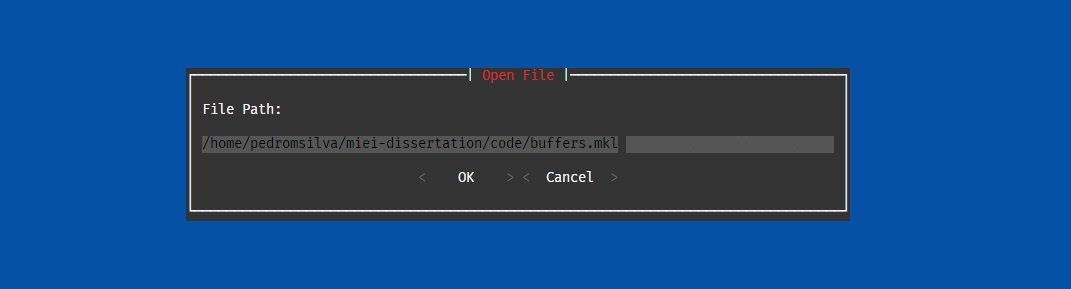
\includegraphics[width=0.87\textwidth]{img/open_buffers_dialog.png}
\end{center}
\caption{Janela de carregamento dos buffers}
\end{figure}

Os conteúdos do \textit{buffer} são guardados num ficheiro \texttt{.mkl}, o que é bastante interessante pois permite evitar ter de criar e implementar algum formato específico para guardar os seus conteúdos. Mas também permite, sendo um formato de texto, e sendo a sua sintaxe a da nossa linguagem \textit{Musikla}, o utilizador pode gravar os \textit{buffers}, abrir o ficheiro com algum editor de texto e efetuar alterações manualmente, e carregar essas alterações de novo para os \textit{buffers} com extrema facilidade.

\begin{lstlisting}[caption={Formato do ficheiro de gravação dos \textit{buffers}.}]
$buffers = @{};
$buffers::set(1; (:default r2/23 [B^d^f]1/29 r1/32 [A^ce]1/32))
\end{lstlisting}

O formato do ficheiro passa pela declaração de uma variável \textbf{\$buffers} contendo um dicionário. O dicionário contém depois um par chave-valor para cada \textit{buffer} não vazio aquando da gravação do ficheiro. A chave representa o índice do \textit{buffer}, e o valor representa a sequência músical lá guardada nesse momento.

Para guardar o ficheiro, é criada é memória a sua \acrshort{ast} respetiva. Esta é depois convertida em texto através da classe \texttt{CodePrinter}.

O processo de carregar o ficheiro é igualmente simples, passando por executar o \textit{script} num contexto isolado. Depois o valor da variável \texttt{\$buffers} é obtido, e as entradas do dicionário são percorridas, substituindo os valores presentes nos \textit{buffers} recorrendo á funcção \texttt{keyboard\textbackslash{}Buffer.from\_music()}.

\subsection{Grelhas}
\subsection{Transformadores}
\subsection{Editor Embutido}

